\RequirePackage[l2tabu, orthodox]{nag}
\documentclass[a4paper, twocolumn]{article}
\usepackage[utf8]{inputenc}
\usepackage[T1]{fontenc}
\usepackage[pdftex, hidelinks,
            pdftitle={Behaviour Tree Evolution by Genetic Programming},
            pdfauthor={Martin Estgren and Erik S. V. Jansson},
            pdfsubject={Artificial Intelligence - Genetic Programming},
            pdfkeywords={artificial intelligence, genetic programming,
                         behaviour trees, a-star, shooter}]{hyperref}

\usepackage{bm}
\usepackage{caption}
\usepackage{listings}
\usepackage{booktabs}
\usepackage{mathtools}
\usepackage{algorithmic}
\usepackage{graphicx}
\usepackage{courier}
\usepackage{amsmath}
\usepackage{amssymb}
\usepackage{algorithm}
\usepackage[capitalize, noabbrev]{cleveref}
\usepackage[activate={true, nocompatibility}, final,
            tracking=true, kerning=true, spacing=true,
            factor=1100, stretch=10, shrink=10]{microtype}

\DeclareCaptionFormat{modifiedlst}{\rule{\textwidth}{0.85pt}\\[-2.9pt]#1#2#3}
\captionsetup[lstlisting]{format =  modifiedlst,
labelfont=bf,singlelinecheck=off,labelsep=space}
\lstset{basicstyle=\footnotesize\ttfamily,
        breakatwhitespace = false,
        breaklines = true,
        keepspaces = true,
        language = Java,
        showspaces = false,
        showstringspaces = false,
        frame = tb,
        numbers = left,
        numbersep = 5pt,
        xleftmargin = 16pt,
        framexleftmargin = 16pt,
        belowskip = \bigskipamount,
        aboveskip = \bigskipamount,
        escapeinside={<@}{@>}}

\title{\textbf{Behaviour Tree Evolution by Genetic Programming}\\
       \Large{\emph{-- Learning Novel Bot Behaviours in a 2D Top-Down Arena Shooter --}}}
\author{{\textbf{Martin Estgren}} \;\;\;\;\;\;\;\;\;\, {\href{mailto:mares480@student.liu.se}
                                                       {\texttt{<mares480@student.liu.se>}}} \\
        {\textbf{Erik S. V. Jansson}} \;\;\;\;         {\href{mailto:erija578@student.liu.se}
                                                       {\texttt{<erija578@student.liu.se>}}} \\~\\
        {Linköping University, Sweden}\vspace{-2.0ex}}

\begin{document}
    \maketitle
    \section*{Abstract}

    Behaviour trees are a popular model for representing the decision-making and plan execution process for NPCs in video games. These are built by hand, and require expertise to craft. They don't adapt well to other environments, and often require a custom BT.

    In this paper we demonstrate how to generate the BTs by using genetic programming; allowing us to essentially evolve novel behaviours automatically in our testbed. Results show that the evolved BT beats our hand-crafted BT by the \(5^{th}\) generation. \footnote{Repository: \url{https://github.com/sci10n/Quake2D}}

    \vspace{1.8em}

    \begingroup
    \def\addvspace#1{}
    \tableofcontents
    \endgroup
    \newpage

    \newpage % Next column...
    \nocite{*} % Include all.
    \bibliographystyle{abbrv}
    \bibliography{report}
    \clearpage

    \section{Introduction} \label{sec:introduction}
	
	Interactive media such as games there is often a need of simulating seemingly complex agent behaviors in realtime. In modern fast-pace computer games for example, the simulation needs to complete one step of the simulation in less than 16ms to provide a half-decent experience. These requirements have spawned some very fast and clever techniques to enable complex behavior for autonomus agents.

	These techniques often requires manual creation and in some cases, are hard to extend when new behaviors are needed for a game \textbf{Cite FSM}. In this project we have explored how one of the more widley hused techniques, \emph{Behavior Trees} can be extended to allow for not only hand crafter complex behaviors, but also for organic behaviors tailored to the specific game domain with the help of \emph{reinforcment learning}.


    \section{Background Theory} \label{sec:background_theory}

	For a autonomus agent to give the illusion of intelligence, many different systems need to interact. In the case of this project, the spatial path-finding and the behavior model has been decoupled where the path-finding system only receives a target position in the simulated environment and left to find the best path to the target by it self.

        \subsection{Behaviour Trees} \label{sec:behaviour_trees}

	

        \subsection{Path Finding with A*} \label{sec:path_finding}

	Agent path finding is done using the \emph{A*} graph traversal algorithm propsed by Peter E. Hart, Nils J. Nilsson, and Bertram Raphael ~\cite{hart1968formal} as an extension to \emph{Dijkstra's algorithm} which, given an \emph{admissible heuristic} and non-negative costs, will find the path from a node \(n_0\) to node \(n_g\) with the lowest cost.
	
	Calculating the expected cost of an path from \(n_0,...,n_k,...,n_g\) can be done as the folowing funcion:
	\begin{equation*}
		f(n_k) = g(n_k) + h(n_k)
	\end{equation*}	
	where \(g(n_k)\) is the true cost from \(n_0\) to node \(n_k\) and \(h(n_k)\) is a heuristic aproximation of the cost from \(n_k\) to \(n_g\).

        In this project, \emph{euclidean distance} is used as the heuristic \(h(n_k)\) since the path-finding is performed in a search-space where each node is defined as a point in the world-space. 

	Additionally to regular \emph{A*}, the pathfinder also utilizes an \emph{influence map} to help the agent avoid suicidal paths, even if the selected path is optimal given the heuristic function. The \emph{influence map} takes into account the visibilty of each node in relation to adversarial game agentss' line-of-sight and updates the expected cost as:
	\begin{equation*}
		f(n_k) = g(n_k) + h(n_k) + i(n_k)
	\end{equation*} 
	which has the result of nodes within adversarial agents line-of-sight having a much higher associated traversial cost. 
	
\begin{minipage}{\linewidth}        	
        \centering
	\begin{minipage}{0.4\linewidth}
	\begin{figure}[H]
		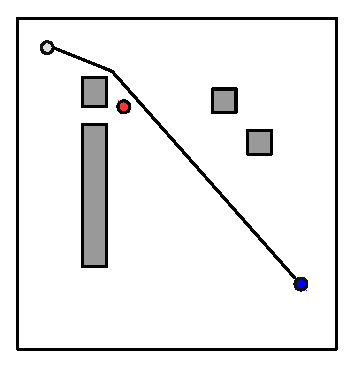
\includegraphics[width=\linewidth]{share/bad.eps}
		\caption{}
		\label{fig:optimal_path}
        \end{figure}
	\end{minipage}
	\hspace{0.05\linewidth}
	\begin{minipage}{0.4\linewidth}
	\begin{figure}[H]
		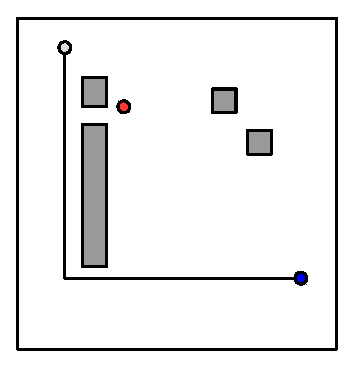
\includegraphics[width=\linewidth]{share/good.eps}
		\caption{}
		\label{fig:smart_path}
	\end{figure}
	\end{minipage}
\end{minipage}
	Above are two example figures, one showing (fig~\ref{fig:optimal_path}) an optimal path using regular \emph{A*}, and the other showing the optimal path when taking into account the influence map (fig~\ref{fig:smart_path}).
	
	\subsection{Genetic Programming} \label{sec:genetic_programming}

	In many scenarios you try to optimize the input of an function \(f(x_0,x_1,...,x_n)\) where some or all of the inputs are of an discreete nature (ordinal or nominal values). These types of problems are often hard to optimize using techniques developed for conitnious variables, such as \emph{gradient ascent/descent}.

	\emph{Genetic programming} is an technique presented by \emph{Nils Barricelli} ~\cite{barricelli1954esempi} as a way to optimize computer programs by encoding with \emph{genetic representation} which could be processed by \emph{evolutionary algorithms}. 

	\begin{figure}[H]
		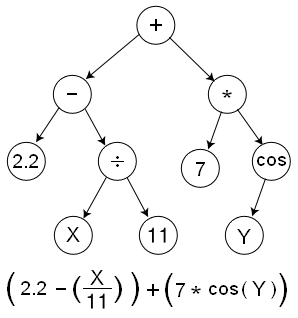
\includegraphics[width=0.8\linewidth]{share/Genetic_Program_Tree.png}
		\caption{The \emph{genetic representation} is often done using a tree structure.}
		\label{fig:genetic_representation}
	\end{figure}

	The typical \emph{evolutionary algorithm} can be described in the following steps.

	Generate inital population where ieach individual as a randomized genetic representation.

	Evaluate fitness for each individual

	Regenerate the poulation using the individuals with the highest fitness from previous generation. The regeneration process i split into several parts, Selection, Breeding, Mutation and Replacment.
	
    \section{Implementation Details} \label{sec:implementation_details}



        \subsection{Game Architecture} \label{sec:game_architecture}


        \subsection{Behaviour Trees} \label{sec:behaviour_trees_implementation}


        \subsection{Genetic Programming} \label{sec:genetic_programming_implementation}



    \section{Results and Screenshots} \label{sec:results_and_screenshots}



        \subsection{Generated Behaviours} \label{sec:generated_behaviours}



        \subsection{Behaviour Fitness} \label{sec:behaviour_fitness}



        \subsection{Survival Rate} \label{sec:survival_rate}



    \section{Discussion and Outlook} \label{sec:discussion_and_outlook}



\end{document}
